% !TEX TS-program = pdflatex
% !TEX encoding = UTF-8 Unicode

\documentclass[11pt, letterpaper]{article}

\usepackage[utf8]{inputenc}
\usepackage[french]{babel}
\usepackage{lmodern}
\usepackage[T1]{fontenc}
\usepackage{amsmath,amsfonts,amsthm,amssymb}
\usepackage{graphicx}
\usepackage{textcomp}

% Dimensions
\usepackage[top=2cm, bottom=2cm, left=1.8cm, right=1.8cm, columnsep=20pt]{geometry}

% graphiques
\usepackage{graphicx}

% PACKAGES
\usepackage{booktabs}
\usepackage{multirow}
\usepackage{tikz}
\usepackage{slashbox}
\usetikzlibrary{automata,positioning}
\begin{document}

\begin{titlepage}
\center

\vspace*{2cm}

\textsc{\LARGE Université de Montréal}\\[1cm] 
\textsc{\Large IFT 3295 -- Bio-Informatique}\\[1.5cm] 

\rule{\linewidth}{0.5mm} \\[0.5cm]
{\LARGE \bfseries Devoir 1} \\[0.2cm] % ***éditez ceci***
\rule{\linewidth}{0.5mm} \\[3cm]
 
\large par: \\*
André Lalonde \\* % ***éditez ceci***
(20024885) \\*[1cm] % ***éditez ceci***
Maude Sabourin \\*
(p1141140) \\*[6cm]
{\large \today}\\[2cm]

\vfill
\end{titlepage}
\newpage
\flushleft
\par{
\textbf{Chevauchement de séquences} \\*[1cm]
\quad 1. Quelle est la différence entre un tel alignement et l'alignement global? \\*[5mm]
\textbf{\underline{Réponse}:} Un tel alignement recherche le meilleur match au travers d'une séquence sans obligatoirement devoir aligner la séquence entière. Ainsi, pour l'alignement global, chaque indel doit être pénalisé peu importe sa position. L'alignement préfixe-suffixe (et inversement) vise plutôt à s'assurer qu'une séquence commence son alignement à partir du début, et qu'une autre complète l'alignement avec la fin de sa séquence. \\*[5mm] Quelles doivent être les valeurs de la première ligne $(V(0,j) \ \forall j)$? et celles de la première colonne $(V(i,0) \ \forall i)$ de la table de programmation dynamique $V$? \\*[5mm]
\textbf{\underline{Réponse}:} Puisque l'alignement permet d'avoir un préfixe et/ou un suffixe, la première rangée ainsi que la première colonne ne contiennent que des 0. Étant donné que l'on n'a aucune restriction par rapport au nombre de caractères qui doivent être "matchés" dans la séquence, on ne pénalise pas un "décalage initiale", puisque l'on peut démarrer de n'importe quelle des deux séquences. \\*[5mm]
\quad 3. Quelles sont les équations de récurrence à utiliser pour remplir la table de programmation dynamique? \\*[5mm]
\textbf{\underline{Réponse}:} Les équations sont \\*[3mm]
\center
\begin{equation}
	max \begin{cases}
	V(i-1,j-1) + : \begin{cases}
									+4 \ si \ v_i = w_j \\
									-4 \ si \ v_i \neq w_j
									\end{cases} \\
	V(i-1,j) - 8 \\
	V(i,j-1) - 8
	\end{cases}
\end{equation} \\*[5mm]
\flushleft
\quad 4. Comment peut-on retrouver l'alignement avec le meilleur chevauchement à partir de la table de programmation dynamique? \\*[5mm]
\textbf{\underline{Réponse}:} Premièrement, on cherche dans le tableau la plus grande valeur sur la dernière ligne ou la dernière colonne, qui sera la case de départ. Par la suite, on vérifie le score de la case sur laquelle on se trouve et les trois cases ($\uparrow, \nwarrow, \leftarrow$) pour s'assurer que le score équivaut bien aux équations de récurrence à gauche. Lorsque l'on se déplace dans la direction $\nwarrow$, les deux case ont un "match" et on écrit donc les deux caractères de la case $V(i,j)$. Lorsque l'on se déplace dans la direction $\uparrow$, alors on "match" le caractère de la ligne $i$ avec un indel. De façon similaire, lorsque l'on se déplace vers $\leftarrow$, alors on "match" le caractère de la ligne $j$ avec un indel. Lorsque l'on arrive sur une case qui vaut 0, on arrête la procédure et on se dirige vers la case $V(0,0)$ en alignant avec des indels le reste de la séquence. \\*[5mm]
\quad 5. Voir le fichier TP1.py. Lancer l'application. Peser sur 1, puis entrez le fichier désiré. Le format fonctionnel est d'écrire une séquence par ligne jusqu'à concurrence de deux.\\
\newpage
\textbf{Assemblage de fragments} \\*[1cm]
\quad 1. Pour chaque paire de reads $\{R_x, R_y \}$, calculer le score de l'alignement correspondant au chevauchement maximal entre $R_x$ et $R_y$. \\*[5mm]
\quad 1.1. Voir le fichier TP1.py. Lancer l'application. Peser sur 2, puis patienter. Une fois toute la recherche effectuée, la matrice s'affichera.
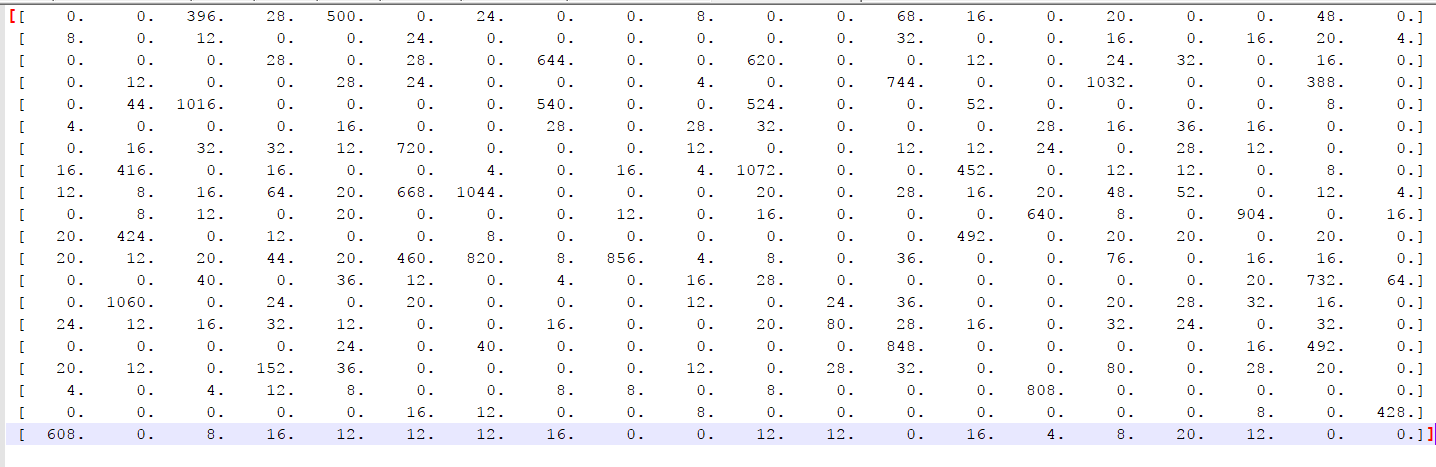
\includegraphics[width=\textwidth]{Images/Matrix_assemblage_no1.png} \\*[5mm]
\quad 2. En déduire le graphe orienté de chevauchement $G = (V,E)$. \\*[5mm]
\centering
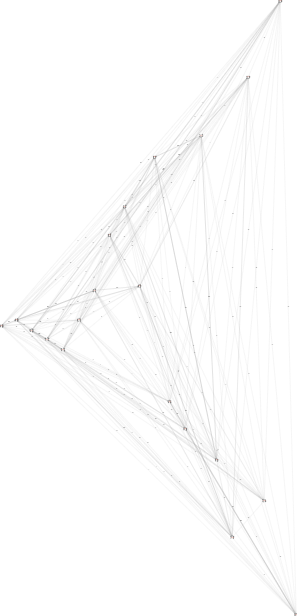
\includegraphics[width=0.25\textwidth]{Images/Assemblage_no2_initial.png}\\*[5mm]
\newpage
\flushleft
a) Quel effet à un seuil minimum de score de 80 sur le graphe résultant? \\*[3mm]
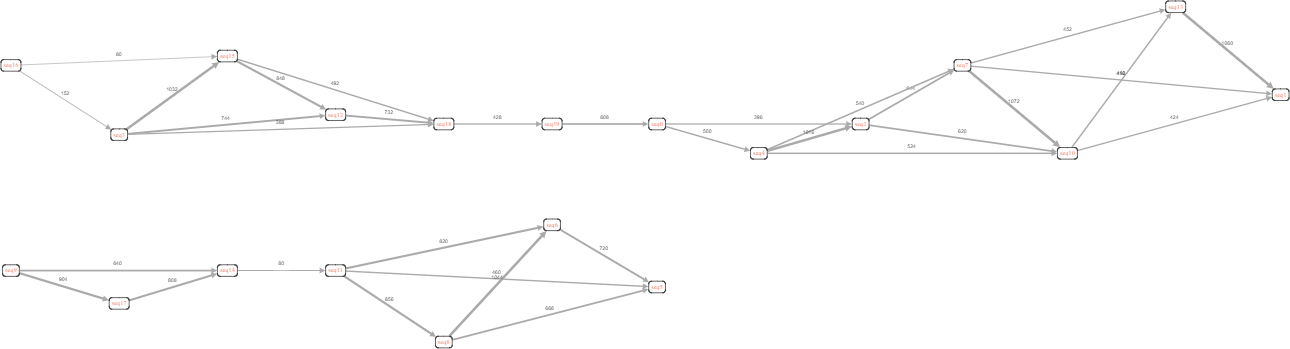
\includegraphics[width=\textwidth]{Images/Assemblage_no2_plus80.png} \\*[3mm]
\textbf{\underline{Réponse}:} Comme on peut le constater en comparant les deux figures précédentes, l'ajout d'un seuil a eu pour effet de diluer la grande majorité des arêtes de $V$. Cela a transformer le \textbf{tas} de séquences en une \textbf{série de séquences} presque linéaire, ce qui nous permet de distinguer les \textbf{patterns} dans les séquences. \\*[3mm]

b) Sachant que le read @READS\_2 est forward, déduisez-en l'ensemble des reads reverse. \\*[3mm]
\textbf{\underline{Réponse}:} L'ensemble des reads reverse est: 5,6,8,9,11,14 et 17. La séparation des reads en deux graphes ne laisse aucun doute sur l'appartenance de chacun à un groupe distinct.\\*[5mm]
\quad 3. a) Construire le nouveau graphe de chevauchement en remplaçant les séquences identifiées comme étant des reads reverse par leur complément $X^r_c$. \\*[3mm]
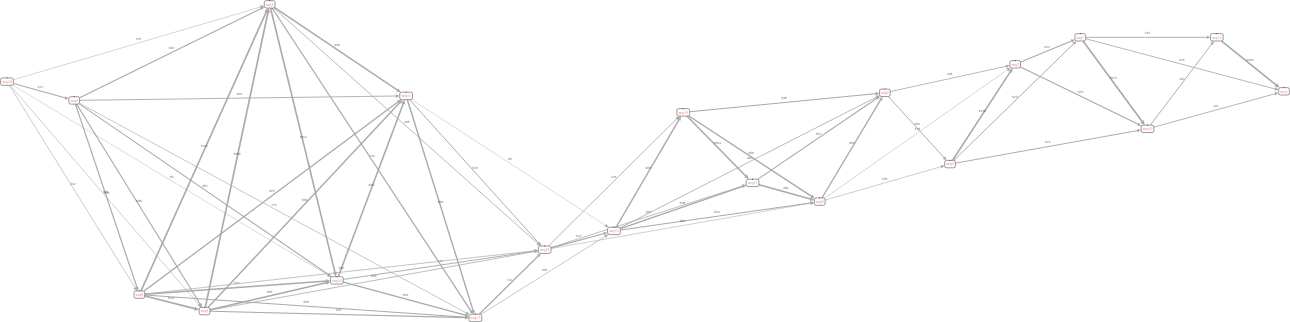
\includegraphics[width=\textwidth]{Images/Assemblage_no3_a).png} \\*[3mm]
Le graphe est maintenant connexe, ce qui veut dire que l'on peut le traverser d'un bout à l'autre par un chemin. De plus, la forme spéciale du graphe aide à voir rapidement les reads qui ont beaucoup de liens.
b) Appliquez la réduction transitive au graphe ci-dessus. \\*[5mm]
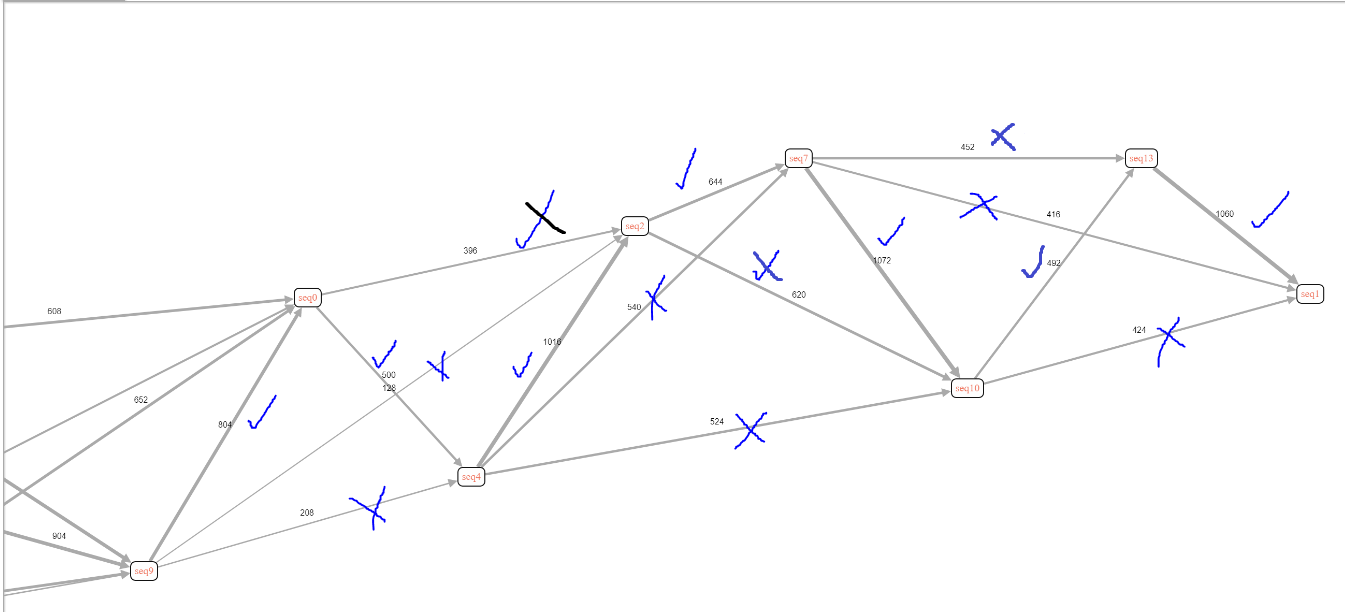
\includegraphics[width=\textwidth]{Images/Reduction_trans_1.png} \\*[5mm]
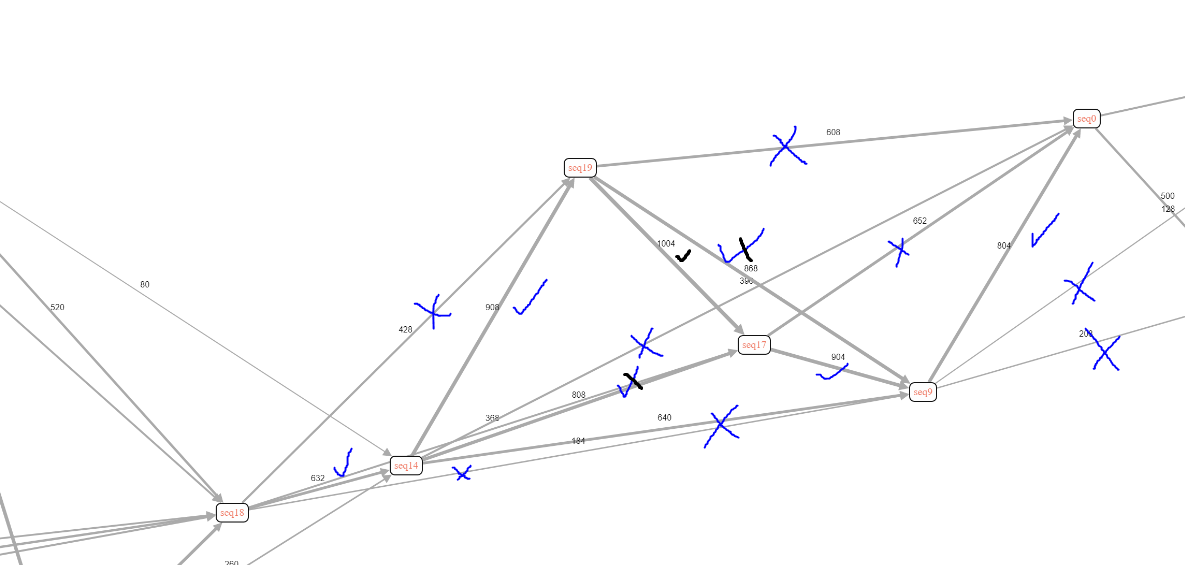
\includegraphics[width=\textwidth]{Images/Reduction_trans_2.png} \\*[5mm]
\newpage
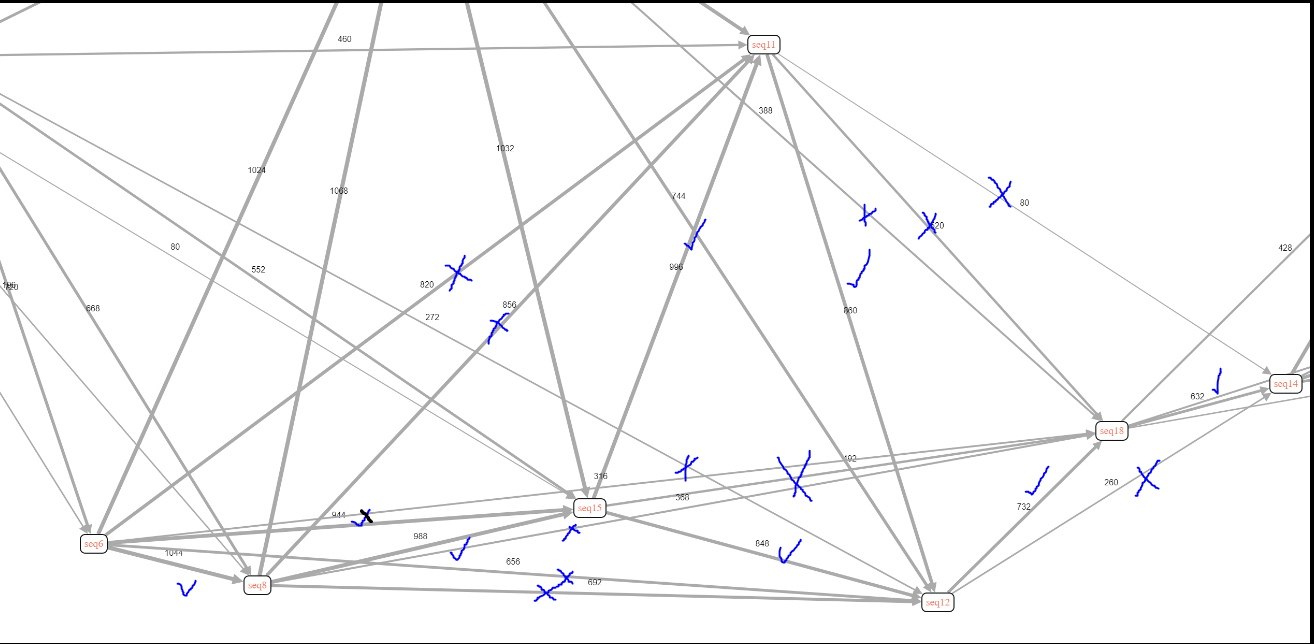
\includegraphics[width=\textwidth]{Images/Reduction_trans_3.png} \\*[5mm]
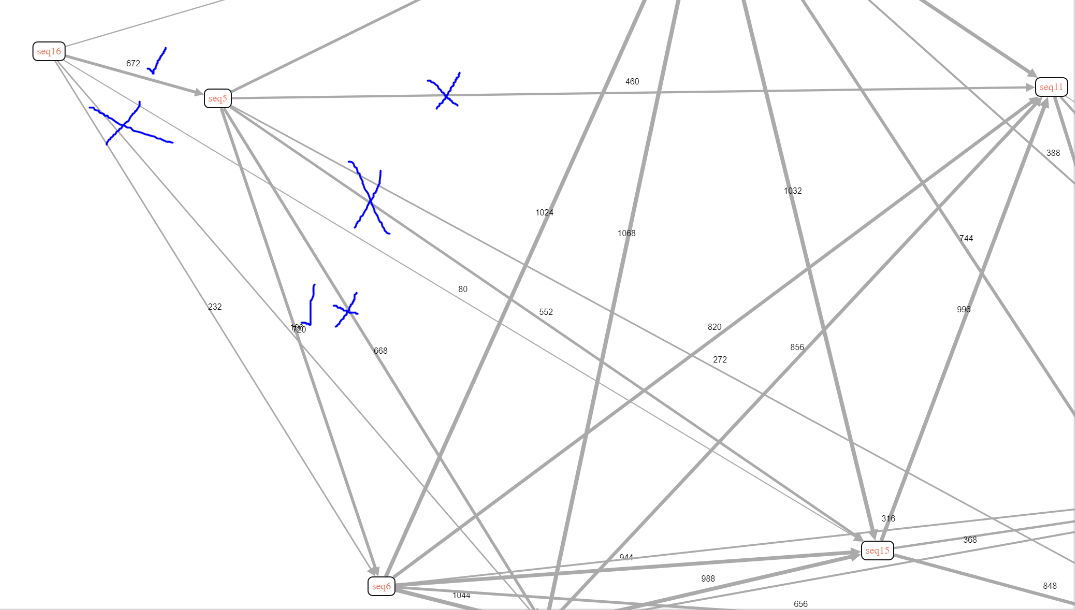
\includegraphics[width=\textwidth]{Images/Reduction_trans_4.png} \\*[5mm]
\newpage
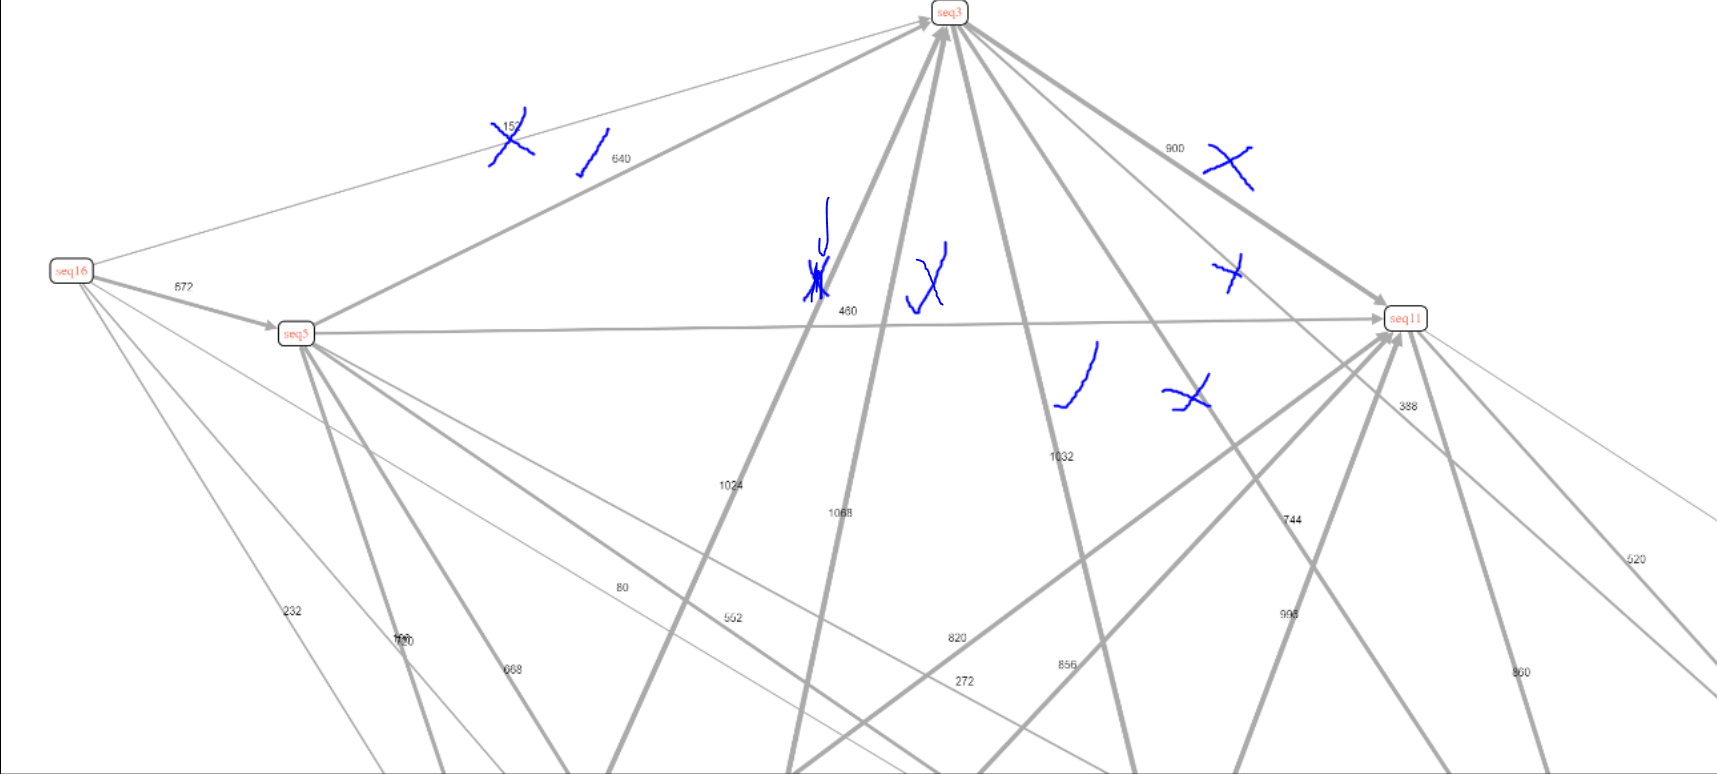
\includegraphics[width=\textwidth]{Images/Reduction_trans_5.png} \\*[5mm]
Ordre des reads : 16->5->6->8->3->15->11->12->18->14->19->17->9->0->4->2->7->10->13->1
Longueur chauvauchment : 
\begin{itemize}
\item Chevauchement 16->5: 174
\item Chevauchement 5->6: 194
\item Chevauchement 6->8: 283
\item Chevauchement 8->3: 293
\item Chevauchement 3->15: 276
\item Chevauchement 15->11: 281
\item Chevauchement 11->12: 247
\item Chevauchement 12->18: 199
\item Chevauchement 18->14: 174
\item Chevauchement 14->19: 243
\item Chevauchement 19->17: 277
\item Chevauchement 17->9: 258
\item Chevauchement 9->0: 225
\item Chevauchement 0->4: 133
\item Chevauchement 4->2: 280
\item Chevauchement 2->7: 169
\item Chevauchement 7->10: 292
\item Chevauchement 10->13: 135
\item Chevauchement 13->1: 281
\end{itemize}
c) Déduire la séquence du fragment génomique séquencé et sa longueur. \\*[3mm]
La séquence est :  CATTCTCCAACCCAGTGATGAGATTGATGATTATAAATGTCACTATCTTCACTGAAAAGTTTAAAGAAATCTTAATGATT\\*[2mm]
ACCAAAATAACTTATCTCTCACTGGAAGAGTTCAAGTGGATTGGCAGCAAATCTGAGATCTATTTGGTGTGACCTGGTGAGATCTAAATATGG\\*[2mm]
AGTCAGCACATGATTTTTTTAAGAGTAATATTGCTAAGTAATATTGCTAAGTATAGTCTGAAAATACCTCTAATCAAAATTATTTACTTGAGAAA\\*[2mm]
AGTATTCAGAATAGTTCCTAAAAATTAAGAGTATATTTCTGGTATAAAAGGATAAATATTCTGT
\\*[2mm]
ATATGAGTATTAATCCAATATGCTTAAAACTTCAGTATTTTACTTAAAAGTACTGTTTGTCATTAAAATTATACCAAAGGTAGAATGCACTTGTTTAATATACTCT
\\*[2mm]
CATGATTCTTTTGCAGGGTGTTCATTTAGAAGAAAGCAACACTAATGATTCAAACAGCTTCCTGAATTTTAATTTTGTGTTGTCTCTC\\*[2mm]
avec une longueur de 526. Les calculs ont été effectués dans le document calculfinal et le résultat complet se trouve dans le fichier totalefinale
\newpage
\textbf{Recherche d'introns et Blast} \\*[1cm]

\quad 1. Identifier la protéine X au sein de la région génomique. \\*[5mm]
 La première étape consiste à prendre le gêne et à le traduire en acides aminés avec la table génétique. Ensuite, on remarque un pattern assez évident.
\includegraphics[width=\textwidth]{Images/gene_comparaison.png} \\*[5mm]
On a donc les informations suivantes : 
\begin{itemize}
\item Extron : MCQRCGLKLIVIICFFVQLARDLLHPSLEEEKKKHKKKRLVQSPNSYFMDVKCPGKI \\*[5mm]
On remarque que la suite du gêne est dans le brin codant 3 
\includegraphics[width=\textwidth]{Images/gene_comparaison2.png} \\*[5mm]
\item Extron : HCLFFFLVCYKITTVFSHAQTVVLCVGCSTVLCQPTGGKARLTEGLSFGILQPSDEIDDYKCLYLH pour le TTVFS jusqu'à KARLTEG \\*[5mm]
Et la fin est dans le brin codant 2
\item Extron : SNILKTSVFYLKVLFVIKIIAKVECTCLIYSHDSFADCSFRRKQH pour le CSFRRKQH \\*[5mm]
\end{itemize}
a) Dans quel cadre de lecture se trouve le codon start de la séquence protéique? \\*[3mm]
\textbf{\underline{Réponse}:} Dans le deuxième brin codant. En effet, on remarque la combinaison ATG(M), suivi de TGC(C), CAG(Q), etc. dans la séquence commençant par GGA\\*[3mm]

b) Décrivez un algorithme de programmation dynamique qui vous permet de retrouver les différents fragments de la protéine X au sein de la séquence nucléotidique. \\*[3mm]
\textbf{\underline{Réponse}:} Nous pouvons utiliser un algorithme d'\textbf{alignement total}. Dès que l'on obtient un mismatch ou un indel, on assigne cela à \textbf{un intron}. Si l'on doit assigner un extra à gauche ou bien à droite, on l'assigne à \textbf{un extron}. \\*[3mm]
c) En déduire les intervalles de positions contenant les exons ainsi que la séquence de l'ARNm mature. \\*[3mm]
\quad 2. En vous servant de l'outil uniprot, identifiez le nom de la protéine X ainsi que sa fonction. \\*[5mm]
\textbf{\underline{Réponse}:} La protéine en question est une \textbf{Ribosomal protein S27 homo sapiens (Human)}. Elle sert à contraindre des acides désoxyribonucléique ainsi que des acides ribonucléiques dans des ribosomes, ou elle lie des ions de Zinc.
\end{document}